%Cody Lewis, Luke De Ruyter, 2012
%Visit anzhelka.com for all the latest
%
% CTRL+SPACE to switch panes in Texmaker
%
% Note: blank lines indicate a new paragraph
% Note: \left( and \right) cannot break lines.

% TODO: Additional material
% --- Section 2.1 still needs more content

% Needs approval and over sight from Cody :)


\documentclass[english]{article}

% Packages that are being used.
\usepackage{amsmath}
\usepackage{longtable}
\usepackage{color}
%\usepackage{verbatim} % used to display code
\usepackage{listings}
\usepackage{graphicx}
\usepackage{subfigure}
\usepackage{indentfirst}
\usepackage{fancyhdr} % Fancy Header
\usepackage{rotating} % To make vertical text in tables
\usepackage[normalem]{ulem} %for strikethroughs

\usepackage{enumerate} % For letter/number list

%\usepackage{babel}

%\usepackage{hyperref} %Must be at the end of use package but before "other settings". Used to make links of all references.




\numberwithin{equation}{section} %change the numbering to have something like 1.1 and 3.15, etc.
%Format of macro:
%\newcommand{\NAME}[ARGUMENT NUMBER (OPTIONAL)]{ stuff to include, arguments denoted #1, #2, etc. }
\newcommand{\vect}[1]{\boldsymbol{#1^2}}
\newcommand{\bigvect}[3]{\boldsymbol{#1^#2^#3}}
\newcommand{\bs}[1]{\boldsymbol{#1}}

%\addto{\captionsenglish}{\renewcommand*{\appendixname}{MyAppx}}

\definecolor{lightlightgray}{gray}{0.9}

\graphicspath{{../tests/}{../figures/}{../extra/}{../figures/editorial/}} %\graphicspath{{path/one/}{path/two/}{path/three/}}

\fancyhead[RO,RE]{\textit{Page \thepage}}
\fancyhead[CO,CE]{}
\fancyhead[LO,LE]{\textit{Software Requirements Specification for Anzhelka}}
\fancyfoot[CO,CE]{ \thepage \\ 
\includegraphics[width=2cm]{../extra/pheonix_small.png}}
\pagestyle{fancy}

\setcounter{tocdepth}{1} %display only sections in table of contents

\begin{document}

\pagenumbering{roman}

\lstset{
%language=C,                             % Code langugage
basicstyle=\ttfamily,                   % Code font, Examples: \footnotesize, \ttfamily
keywordstyle=\color{OliveGreen},        % Keywords font ('*' = uppercase)
commentstyle=\color{gray},              % Comments font
%numbers=left,                           % Line nums position
%numberstyle=\tiny,                      % Line-numbers fonts
%stepnumber=1,                           % Step between two line-numbers
%numbersep=5pt,                          % How far are line-numbers from code
backgroundcolor=\color{lightlightgray}, % Choose background color
frame=none,                             % A frame around the code
tabsize=4,                              % Default tab size
captionpos=b,                           % Caption-position = bottom
breaklines=true,                        % Automatic line breaking?
breakatwhitespace=false,                % Automatic breaks only at whitespace?
showspaces=false,                       % Dont make spaces visible
showtabs=false,                         % Dont make tabls visible
%columns=flexible,                       % Column format
%morekeywords={__global__, __device__},  % CUDA specific keywords
}







%\\ Version 1.0 approved \\ Prepared by Luke De Ruyter, Cody Lewis \\ University of California, Riverside \\ \date{\today}
\title{\begin{flushright}\textbf{
\rule{\textwidth}{3 pt} \\
\bigskip \bigskip
\Huge Software/Hardware \\ 
Requirements Specification \\ 
\bigskip \LARGE for \\ \bigskip
\Huge Anzhelka \\
\bigskip \bigskip \bigskip
\large Version 1.0 approved \\
\bigskip \bigskip \bigskip
Prepared by \\ Luke De Ruyter \\Cody Lewis \\
\bigskip \bigskip \bigskip
University of California, Riverside \\
\bigskip \bigskip \bigskip
\today
}\end{flushright}}
%\author{Cody Lewis \\ \texttt{srlm@anzhelka.com} \and Luke De Ruyter \\ \texttt{ilukester@anzhelka.com} }
%\date{\today}
\date{}
\author{}
\maketitle 
\newpage

%\begin{center}
\includegraphics[scale=.24]{tribal_phoenix.jpg}\end{center}

%% TOC TOC TOC TOC TOC TOC TOC TOC TOC TOC TOC TOC
\renewcommand{\contentsname}{Table of Contents}
\tableofcontents
%\addcontentsline{toc}{section}{Table of Contents}
%% TOC TOC TOC TOC TOC TOC TOC TOC TOC TOC TOC TOC


%% REV REV REV REV REV REV REV REV REV REV REV REV REV
\section*{Revisions}
Current project status and files can be found at
\begin{center}
 \textbf{blog.anzhelka.com} \\
 \textbf{code.anzhelka.com} \\
\end{center}

\begin{longtable}{l | l | p{5cm} | l}
\hline
\textbf{Version} & \textbf{Date} & \textbf{Changes} & \textbf{Commiter}\\
\hline
0.01	& April 30, 2012 & Initial layout of file was created. 	& Cody \\
\hline
0.02	& May 4, 2012 & Purpose, Audience, Scope, Perspective, Functions, and Users was populated. & Cody, Luke \\
\hline
\end{longtable}

%% REV REV REV REV REV REV REV REV REV REV REV REV REV


\newpage
\pagenumbering{arabic}


%% S1 S1 S1 S1 S1 S1 S1 S1 S1 S1 S1 S1 S1 S1 S1 S1 S1 S1 S1 S1  

%% S1 S1 S1 S1 S1 S1 S1 S1 S1 S1 S1 S1 S1 S1 S1 S1 S1 S1 S1 S1  

%% S1 S1 S1 S1 S1 S1 S1 S1 S1 S1 S1 S1 S1 S1 S1 S1 S1 S1 S1 S1  
\section{Introduction}
\subsection{Purpose}
Anzhelka is a complete system intended for autonomous quadrotor flight. Included as a part of Anzhelka is both hardware and software. This includes the quadrotor frame, control electronics, ground station software, and the complete system documentation. Anzhelka is completely open source, and all project files are available for download. You can find in this document any instructions necessary for understanding the functionality of Anzhelka components. This includes hardware and software interfaces, features, and system requirements.
\subsection{Document Conventions}
\subsection{Intended Audience and Reading Suggestions}
This document is written for Anzhelka developers. This document is intended to refine development direction, and to bring new developers up to speed. For this document, developers include software writers, hardware designers, and system testers. When the word "you" is written, it is referring to the developer who is reading this document. When the words "the user" is written, it is referring to the end user of the Anzhelka platform.

You should read this document based on your background with Anzhelka. Current developers can find the appropriate section to read. New developers should read the introduction, overall description, and system features sections. If you are a non-developer for this project, and don't intend to ever become one, you should avoid this document. Look on the Anzhelka website for something more appropriate to your needs.


\subsection{Product Scope}
Anzhelka consists of four main components: a quadrotor hardware frame, custom quadrotor software, ground station software, and detailed documentation via the Anzhelka website. Even without a degree in control systems, you can use Anzhelka components to make an autonomous quadrotor system. By using these components you can customize the functionality of the system to suit your needs, or use them directly to perform predefined commands.


\subsection{References}

\newpage
\section{Overall Description}
\subsection{Product Perspective}

\begin{figure}[h!]
  \centering
	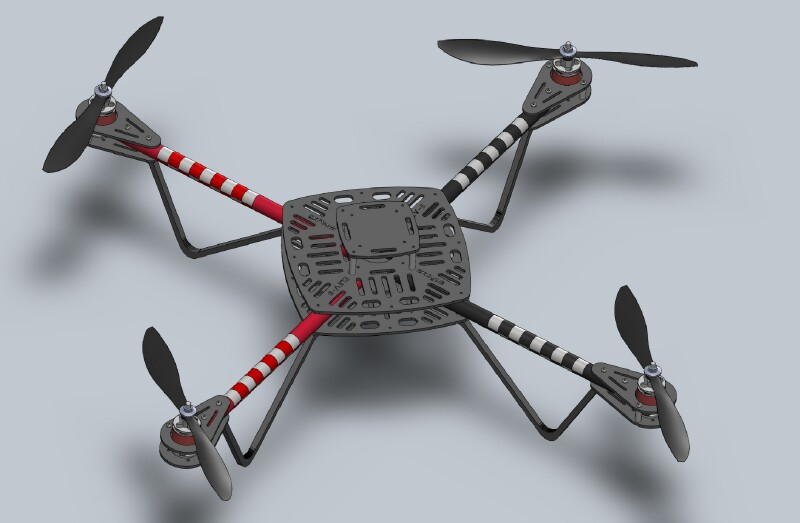
\includegraphics[scale=.6]{elev_8_rendering.JPG}
  \caption{This is an artistic rendering of the frame used for Anzhelka.}
\end{figure}  
Anzhelka is a platform for experimentation in aerial robotics. It is an independent project designed from the ground up. We are taking an existing open hardware frame as our base hardware platform. We have chosen to build on top of this hardware because of its expandability and its durability. We have designed a custom control board that will be able to run all of Anzhelka's software and house all the necessary components.\\
%
%
%\textit{<Describe the context and origin of the product being specified in this SPECIFICATION. For example, state whether this product is a follow-on member of a product family, a replacement for certain existing systems, or a new, self-contained product. If the SPECIFICATION defines a component of a larger system, relate the requirements of the larger system to the functionality of this software or hardware and identify interfaces between the two. A simple diagram that shows the major components of the overall system, subsystem interconnections, and external interfaces can be helpful.>}


\subsection{Product Functions}
Anzhelka is designed to be programmatically controllable in a number of different aspects. The quadrotor can receive commands to set any of it's internal registers, which then affect the flight of the quadrotor. In addition, the quadrotor has a command interpreter that is able to read command sequences from onboard memory. With these commands, the user can control a number of quadrotor functions including attitude and position.

Anzhelka is equipped with a Parallax Propeller multicore processor. The quadrotor has two separate batteries. One battery provides power for the motors and servos; the other battery powers the electronics. The electronic hardware is designed with expandability in mind. The motors and servos have voltage and current monitoring. The Anzhelka system is designed to allow for the easy attachment of additional electronics.

\subsection{User Classes and Characteristics}
%\textit{<Identify the various user classes that you anticipate will use this product. User classes may be differentiated based on frequency of use, subset of product functions used, technical expertise, security or privilege levels, educational level, or experience. Describe the pertinent characteristics of each user class. Certain requirements may pertain only to certain user classes. Distinguish the most important user classes for this product from those who are less important to satisfy.>}

\subsubsection{User Example: Jason}

\begin{figure}[h!]
  \centering
	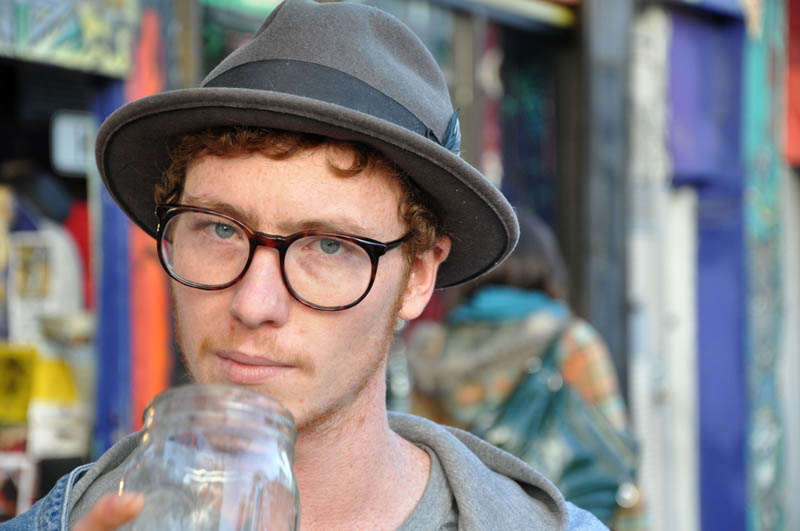
\includegraphics[width=3in]{hipster1.jpg}
  \caption{Jason Lariart}
\end{figure}

\textbf{ Age:} 28

\textbf{ Education:} Some College

\textbf{ Marital Status:} Open

\textbf{ Occupation:} Videographer

\textbf{ Hobbies:} Photography, Videography, Art, Protesting

\textbf{About Jason:} He is an avid videographer and likes to push the limits of his skills, crew, and equipment. He likes to take pictures and videos of things that not just any ordinary person can do. Jason is currently an amateur photographer, but wants to make a professional career out of his work.
\\

\textbf{Scenario:} Jason is preparing for a remote video shoot and realized that he won't be able to get his aerial shot because a helicopter is out of his budget. Jason told the client that he was going to have to spend more money if wanted to get the aerial shot as planned. The client was upset to hear about this and had no choice but to drop the scene from the shoot. %  programmed it so he was able to acchieve the same effect he was looking for while staying in the budget.

\newpage
\subsubsection{User Example: Dan}

\begin{figure}[h!]
  \centering
	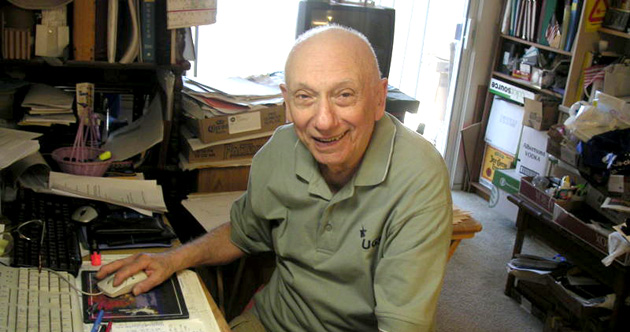
\includegraphics[width=3in]{oldgradstudent.jpg}
  \caption{Dan Knuth}
\end{figure}
\textbf{ Age:} 82

\textbf{ Education:} Doctorate in Mathematics

\textbf{ Marital Status:} Widowed

\textbf{ Occupation:} Software Developer

\textbf{ Hobbies:} Open source programming, online forum posting, sitting

\textbf{About Dan:} Dan works on open source systems. He has literally been around since the begining, and he remembers the days of punch card programming. Throughout his career he has been a strong supporter of making computer science more accessible, and his work in the open source field is both notable and well respected.
\\
\textbf{Scenario:} Dan wants to spend more time focusing on his hobbies, but he doesn't have much time left and he needs to eliminate routine activities. Dan wants to develop a robot to automatically pick up his medicine from the pharmacy and carry it to him. This robot needs to be able to fly, and to be user programmable. Dan has lots of experience in working with software, so it's ok if the product is a bit rough and requires the use of a command line. Dan would be particularly appreciative if the instructions could be programmed in by a series of toggle switches and incandescent lights.

\subsection{Operating Environment}
\subsection{Design and Implementation Constraints}
\subsection{User Documentation}
\subsection{Assumptions and Dependencies}

\newpage
\section{External Interface Requirements}
\subsection{User Interfaces}
\subsection{Hardware Interfaces}
\subsection{Software or Hardware Interfaces}
\subsection{Communications Interfaces}

\newpage
\section{System Features}

This section describes Anzhelka features, and assigns priorities to each. Priorities are assigned in descending order, with a priority of 1 being the most important.

\subsection{Attitude Control}
\subsubsection{Description and Priority}
An quadrotor must be able to maintain a stable attitude (orientation) at all times during flight. If the quadrotor loses control of it's attitude then catastrophic failure is certain to happen. Such a failure would likely result in the destruction of the vehicle, and possibly collateral damage. Therefore, attitude control is \textit{the} top priority of Anzhelka.

\textbf{Priority:} 1

\textbf{Business Requirement:} Allow the user to have a precisely orientable platform

\subsubsection{Stimulus/Response Sequences}

\begin{longtable}{p{3cm} | p{8.5cm}}
\hline
\textbf{Stimulus} & \textbf{Response}\\
\hline
1. Hit By High Velocity Paintballs &
\begin{enumerate}[(a)]\itemsep1pt %for small alpha-characters within brackets.
\item Paintball hits, creates sudden attitude disturbance
\item Quadrotor loses altitude, increase in attitude error
\item Attittude mathematical control loop gains change to compensate
\item Quadrotor adjusts motor speed based on control loop result
\item Quadrotor achieves desired attitude
\end{enumerate}
\\ 
\hline
\end{longtable}
\subsubsection{Functional Requirements}
Attitude control assumes that the quadrotor has sufficient thrust in each motor to maintain a given attitude. In addition, the quadrotor must have a valid desired attitude to work towards. If there is a disturbance to the attitude the quadrotor must be able to correct it's orientation quickly before it changes it's position enough to risk collision.
\bigskip
\subsection{Altitude Control}
\subsubsection{Description and Priority}
Altitude control refers to the ability of the quadrotor to maintain a set height above ground level. This can be sensed through a number of different methods, but each must have the same result. Altitude control is important in order to prevent the quadrotor from crashing to the ground or going too high. Altitude control failure can result in damage to the vehicle or nearby objects, hence altitude control is very important.

\textbf{Priority:} 2

\textbf{Business Requirement:} Gives the user the ability to set a desired altitude for flight

\subsubsection{Stimulus/Response Sequences}

\begin{longtable}{p{3cm} | p{8.5cm}}
\hline
\textbf{Stimulus} & \textbf{Response}\\
\hline
1. Altitude drops by 5cm &
\begin{enumerate}[(a)]\itemsep1pt %for small alpha-characters within brackets.
\item Quadrotor loses 5cm in altitude
\item Altitude sensor on the quadrotor triggers an alarm within control loop
\item Altitude mathematical control loop gains change to compensate
\item Quadrotor adjusts motor speed based on control loop result
\item Quadrotor achieves desired altitude
\end{enumerate}
\\ 
\hline
\end{longtable}
\subsubsection{Functional Requirements}
Altitude hold assumes that the quadrotor can produce enough thrust to maintain the desired altitude. Maximum thrust may not be enough when a)the quadrotor is overloaded and too heavy or b)the quadrotor is flying at a severe angle. If either of these cases are true, then the quadrotor should be expected to lose altitude.
\bigskip
\subsection{Highly Maneuverable}
\subsubsection{Description and Priority}
One of the main advantages of an \textit{autonomous} quadrotor is that the computer control should allow for aerial acrobatics. Most human pilots do not have suitable skill to perform complex movements. By allowing for complex manuevers, the quadrotor is able to go through certain obstacles that it may not normally be able to.

This feature is an important reason to select autonomous flight, and hence an important part of the flight experience. It is not, however, necessary for stable flight.

\textbf{Priority:} 3

\textbf{Business Requirement:} Users have the ability to achieve precise aerobatics

\subsubsection{Stimulus/Response Sequences}

\begin{longtable}{p{3cm} | p{8.5cm}}
\hline
\textbf{Stimulus} & \textbf{Response}\\
\hline
1. Quadrotor is programmed to do a barrel roll &
\begin{enumerate}[(a)]\itemsep1pt %for small alpha-characters within brackets.
\item Quadrotor is instructed to perform a barrel roll
\item Current IMU and Altitude readings are stored
\item The trajectory of the roll is calculated by the barrel roll function
\item Motors are changed to the desired speeds calculated by the control loop
\item Motor speeds are adjusted throughout the duration of the roll to maintain control
\item The Quadrotor is then returned back to the starting attitude and altitude.
\end{enumerate}
\\ 
\hline
\end{longtable}
\subsubsection{Functional Requirements}
The quadrotor must be able fly at any specified orientation. The quadrotor is not expected to maintain position while in an acrobatic movement state. The system should be able to perform these movements with either a human pilot or through a programmable interface.





\bigskip
\subsection{User Programmable}
\subsubsection{Description and Priority}
The quadrotor must be able to accept commands from the user in some relatively conceptually high level format. This allows for users to make the best use of the autonomous features of the quadrotor vehicle.

\textbf{Priority:} 3

\textbf{Business Requirement:} Makes the quadrotor unique to the users needs.

\subsubsection{Stimulus/Response Sequences}

\begin{longtable}{p{3cm} | p{8.5cm}}
\hline
\textbf{Stimulus} & \textbf{Response}\\
\hline
1. The user wants to program the quadrotor with a new trajectory plan &
\begin{enumerate}[(a)]\itemsep1pt %for small alpha-characters within brackets.
\item The user plugs the SD card into a computer
\item The user launches the programming software
\item Trajectories are entered into the software
\item When the user is ready they can press the "Write to SD Card" Button
\item The user then plugs the SD card into the quadrotor
\end{enumerate}
\\ 
\hline
\end{longtable}
\subsubsection{Functional Requirements}
The quadrotor should be programmable in an easy to understand scripting language type format, in plain text. The user program should be able to be stored onboard the quadrotor, and edited on most computers. The scripting language developed should be able to support advanced features such as condition testing and branching. In addition, there should be a graphical user interface to allow for automated programming of the quadrotor.
\bigskip

\subsection{Comprehensive Datalogging}
\subsubsection{Description and Priority}
The quadrotor should document and log all of it's internal parameters and measurements for later review. This is especially important for debugging and assessing system stability. Every number should be stored on a relatively secure and crash-safe memory device. This is important for debugging intermittent errors of the system, and hence is relatively important.

\textbf{Priority:} 3

\textbf{Business Requirement:} Know how the system performed and how to better achieve the desired actions

\subsubsection{Stimulus/Response Sequences}

\begin{longtable}{p{3cm} | p{8.5cm}}
\hline
\textbf{Stimulus} & \textbf{Response}\\
\hline
1. The user wishes to log all flight data &
\begin{enumerate}[(a)]\itemsep1pt %for small alpha-characters within brackets.
\item The user locates the logging switch on the control board
\item The user toggles the switch into the logging position
\item Recording begins once the quadrotor has been initialized
\end{enumerate}
\\ 
\hline
\end{longtable}
\subsubsection{Functional Requirements}
The data should be stored onboard the quadrotor, preferably in a removable medium such as an SD card. The data should also be stored in a plain text file on the medium in order to allow for a wide range of software to process the data.
\bigskip

\subsection{Modularized} 
\subsubsection{Description and Priority}
The quadrotor must be able to be easily assembled and disassembled. This is especially important when the quadrotor is expected to crash frequently. However, as the project matures, development of the quadrotor frame can minimize the modularity of the frame with the expectation of fewer crashes.

\textbf{Priority:} 4

\textbf{Business Requirement:} Interchangeable parts makes a reliable system

\subsubsection{Stimulus/Response Sequences}

\begin{longtable}{p{3cm} | p{8.5cm}}
\hline
\textbf{Stimulus} & \textbf{Response}\\
\hline
1. The user wants to fix one of the motor booms &
\begin{enumerate}[(a)]\itemsep1pt %for small alpha-characters within brackets.
\item The motor mount is removed from the damaged boom
\item The broken motor boom is then removed from the frame
\item A new replacement motor boom is mounted on the frame
\item The motor mount is reattached to the boom
\end{enumerate}
\\ 
\hline
\end{longtable}
\subsubsection{Functional Requirements}
The quadrotor should use threaded fasteners for all joints. The use of glues and other adhesives should be minimized. All fasteners must use the same head and thread sizes to minimize the number of different tools required. All components should be easy to manufacture or inexpensive to purchase, and be easily removable and replaceable when necessary.

\bigskip
\subsection{Ground Station}
\subsubsection{Description and Priority}
A ground station allows the quadrotor operator to view realtime statistics about the operation of the vehicle. Operational data is transmitted wirelessly to a receiver that is connected to a laptop computer for display. The data can include both measured data (such as motor speed or battery level) and calculated data (such as orientation error or next command). While useful and informative, this feature is not required for every flight.

\textbf{Priority:} 4

\textbf{Business Requirement:} Know what the quadrotor is doing while it is doing it

\subsubsection{Stimulus/Response Sequences}

\begin{longtable}{p{3cm} | p{8.5cm}}
\hline
\textbf{Stimulus} & \textbf{Response}\\
\hline
1. The user wants to get data from the quadrotor in real time &
\begin{enumerate}[(a)]\itemsep1pt %for small alpha-characters within brackets.
\item The ground station software is initialized on a computer
\item The user sets the switch labeled "wireless" on the control board to on
\item The ground station hardware is then plugged into the USB port on the computer
\end{enumerate}
\\ 
\hline
\end{longtable}
\subsubsection{Functional Requirements}
The ground station should be self contained, and be available in on of two forms: a small USB device, or a tripod mounted and motorized device. The USB version of the ground station should be able to receive a signal from the quadrotor when it is operating in close proximity, and transmit packets to the quadrotor. The tripod mounted ground station must be able to track the quadrotor with a directional antenna, and also be powered from a USB port.

\bigskip
\subsection{Waypoint Control}
\subsubsection{Description and Priority}
The quadrotor should be able to follow a set waypoint path in 3D space. This allows for precise control of quadrotor position, and can be used for tasks such as surveillance or transportation of payloads. The waypoints should be able to be defined both statically, before flight begins, and dynamically, after flight begins.

\textbf{Priority:} 4

\textbf{Business Requirement:} Allows the user to be able to monitor an area continuously

\subsubsection{Stimulus/Response Sequences}

\begin{longtable}{p{3cm} | p{8.5cm}}
\hline
\textbf{Stimulus} & \textbf{Response}\\
\hline
1. The user wants to control the quadrotor to fly in an continuous pattern &
\begin{enumerate}[(a)]\itemsep1pt %for small alpha-characters within brackets.
\item While using the configuration software the user selects the waypoint tab
\item The user then selects the waypoint pattern
\end{enumerate}
\\ 
\hline
\end{longtable}
\subsubsection{Functional Requirements}
The quadrotor should be able to track it's current position and travel to a specified waypoint. The quadrotor should consider itself at the waypoint once it has reached an distance error radius from the waypoints. The waypoint specification must allow for both a two dimensional specification and a full three dimensional specification. In the case of two dimensions, the quadrotor should maintain it's current position in the unspecified dimension.
% Wouldn't it be cool to have a specification of 1-3 dimensions?

\bigskip
\subsection{Object Tracking}
\subsubsection{Description and Priority}
The quadrotor should be able to track objects in it's immediate environment. This is useful for both avoiding obstacles and tracking the movement of a target. This is especially important when flying in a restricted area such as a forest or urban setting. Should the quadrotor fail to accurately track and avoid objects it will likely hit something, leading to a crash. While this is a serious issue, it is reasonable to expect most flights to take place in an open area, in which case most users would not need object avoidance.

\textbf{Priority:} 5

\textbf{Business Requirement:} The ability to follow an object with an unknown trajectory

\subsubsection{Stimulus/Response Sequences}

\begin{longtable}{p{3cm} | p{8.5cm}}
\hline
\textbf{Stimulus} & \textbf{Response}\\
\hline
1. The user wants to enable the object avoidance software &
\begin{enumerate}[(a)]\itemsep1pt %for small alpha-characters within brackets.
\item The user locates the Object Avoidance switch on the control board
\item The user toggles the switch into the ON position
\end{enumerate}
\\ 
\hline
\end{longtable}
\subsubsection{Functional Requirements}
The object tracking feature must be able to create at least a two dimensional map of the surrounding area, out to within three seconds of travel at the current speed. This map must be updated at least two times per second.


\bigskip
\subsection{Intuitive User Control}
The quadrotor must have a manual flight capability. Ideally, this would be done through an intuitive user interface that does not require much training or experience to operate. Practically this is a low priority requirement since the quadrotor must be operable manually, but this control need not be \textit{intuitive} for early adopters.

\textbf{Priority:} 6

\textbf{Business Requirement:} Gives the user the ability to fly the quadrotor with no fly experience
 
\subsubsection{Description and Priority}
\subsubsection{Stimulus/Response Sequences}

\begin{longtable}{p{3cm} | p{8.5cm}}
\hline
\textbf{Stimulus} & \textbf{Response}\\
\hline
1. The user wants to control the quadrotor manually, without programming flight data &
\begin{enumerate}[(a)]\itemsep1pt %for small alpha-characters within brackets.
\item The user locates the manual flight switch on the control board
\item The user toggles the switch into the manual position
\item The remote flight control board is then able to control the orientation and altitude of the quadrotor
\end{enumerate}
\\ 
\hline
\end{longtable}
\subsubsection{Functional Requirements}
The user must be able to have complete control of the orientation of the quadrotor body, and the z axis thrust produced by the quadrotor. The user control must be wireless and not require any connection to external electronics. The user controller should allow for rapid spinning of the quadrotor body.

\bigskip

\subsection{Open Community Support}
A good open source product must have a central location to store user generated technical support. Forums are one of the best methods available, and reduce the support burden of Anzhelka developers. However, forum based support is only useful once a community of users has been established.

\textbf{Priority:} 7

\textbf{Business Requirement:} An open community means open and free support
\subsubsection{Description and Priority}
\subsubsection{Stimulus/Response Sequences}

\begin{longtable}{p{3cm} | p{8.5cm}}
\hline
\textbf{Stimulus} & \textbf{Response}\\
\hline
1. The user has a problem with troubleshooting a problem with the quadrotor. &
\begin{enumerate}[(a)]\itemsep1pt %for small alpha-characters within brackets.
\item The user browses to our forums website at forums.anzhelka.com
\item The user then selects the appropriate forum, based on the problem
\item The user then log in or create a new account
\item Click on the "Create a new Thread" button
\item In title box the user creates a descriptive title for the problem
\item In the body text box the user enters what the problem is and any troubleshooting that has already been done.
\item The user then posts the thread
\item The user waits for a helpful reply
\end{enumerate}
\\ 
\hline
\end{longtable}
\subsubsection{Functional Requirements}
The forums must be publicly viewable without an account, since most user questions are likely to repeat. The forums must be hosted so that they are accessible from anywhere in the world. In addition, the forums must be moderated, either by users or staff, to ensure a friendly environment free of profanity and politics.


\newpage
\section{Other Nonfunctional Requirements}
\subsection{Performance Requirements}
\subsection{Safety Requirements}
\subsection{Security Requirements}
\subsection{Software or Hardware Quality Attributes}
\subsection{Business Rules}

\newpage
\section{Other Requirements}
\appendix
%\gdef\thesection{Appendix \Alph{section}:}
\section{Glossary}
\section{Analysis Models}
\section{To Be Determined List}


\end{document}
